\section{Model Training}
\subsection{Training Datasets} \label{training data}
In this section, we describe the training datasets used in our two-stage model training. 

\paragraph{Teacher Learning Stage}
In this stage, we use parallel text corpus to align the original CLIP text encoder and our new text encoder initialized from XLM-R. Our parallel text corpus includes the following:
\begin{enumerate}

\item Machine translated data of text in Conceptual Captions (CC3M) ~\cite{sharma2018conceptual} and a 28M randomly sampled subset from Laion-400M ~\cite{schuhmann2021laion}. For the multilingual model, we use the same setting but fewer 10M subsets from Laion-400M for each language.
\item Human translated data of text from TSL2019 ~\cite{xu2019nlp}, a total number of 5M English to Chinese translations. For the multilingual model, we extracted the same amount for each language. Parallel data in different languages is extracted from the public database OPUS\cite{tiedemann2012parallel}\footnote{https://opus.nlpl.eu}. This type of parallel data provides more accurate translation.

\end{enumerate}

%In the two stages of training we use different types of data, image-text pairs and parallel-text pairs, respectively. In the Teacher Learning stage we use parallel text to "mock" the teacher's behavior, then in the contrastive learning stage we use image-text pairs to train our text encoder to better fit the image encoder.

%\paragraph{Data For Teacher Learning}
%The parallel corpus used in the Teacher Learning stage consists of machine-translated corpus and human-translated corpus. An intuitive idea is to directly use the captions in the image-text pair as the text corpus, because the data distribution is closer to the data of downstream tasks, such data are representative of CC3M\cite{sharma2018conceptual} and COCO. Another type of data that is far away from downstream tasks is the captions of image-text pairs crawled from the Internet. This type of data is often noisy, and the representative is LAION400M\cite{schuhmann2021laion}. On the other hand, human-translated corpus is also an important parallel corpus. This kind of corpus is characterized by more accurate translation. Our training data combines machine-translated corpora CC3M and Laion28M (a randomly sampled subset of LAION400M) and human-translated corpus TSL2019\cite{xu2019nlp}, totaling 36M Chinese-English parallel text pairs. Captions often require a neural translation model to translate into the target language, and we translate all the English caption into Chinese by using the translation model \cite{TiedemannThottingal:EAMT2020}.

\paragraph{Contrastive Learning Stage}
We use high-quality text-image pair data in this stage. Note that multilingual data are only used in our multilingual version.
%Our text-image  includes the following:
We use 2M bilingual text-image pairs for AltCLIP and 100M multilingual text-image pairs for the multilingual version, from the following:
\begin{enumerate}
\item Chinese text-image dataset from Wudao MM ~\cite{yuan2021wudaocorpora}, filtered by the Laion Aesthetic v2\footnote{https://github.com/christophschuhmann/improved-aesthetic-predictor} model with a threshold score over 5.5.
\item English text-image dataset from LAION 5B ~\cite{schuhmann2022laion}, a randomly sampled subset from the data filtered by the Laion Aesthstic v2 model with a threshold score over 6.

\item Multilingual text-image dataset from LAION Multilingual 2B ~\cite{schuhmann2022laion}, a randomly sampled subset from the data.
\end{enumerate}
%The total number of text-image pairs we used is 11M. 
%We use a subset of 2M text-image pairs from the above.
%The image-text pair data used in the contrastive learning phase is the parallel pair of Chinese captions and images. At this stage we tend to use higher-quality image-text pair data, and we use the Laion aesthetic model to pick out high-quality image-text pairs. Specifically, we select image-text pairs with an aesthetic score higher than 5.5 points from the Chinese open source multimodal dataset Wudao\cite{yuan2021wudaocorpora} and image-text pairs with an aesthetic score higher than 6 points from Laion Aesthetics v2. A total of 2M image-text pairs are used for comparative learning.

\begin{table*}[hbt]
\centering
\small
\begin{tabular}{ccccccccc}\hline
\multirow{2}{*}{Dataset}   & \multirow{2}{*}{Method} & \multicolumn{3}{l}{Text-to-Image Retrival} & \multicolumn{3}{l}{Image-to-Text Retrival} & \multirow{2}{*}{MR} \\\cline{3-8}
                           &                         & R@1          & R@5          & R@10         & R@1          & R@5          & R@10         &                     \\\hline
\multirow{7}{*}{\rotatebox{90}{Flickr30k$_{EN}$}} & CLIP         &    65.0          &     87.1         &      92.2        &    85.1          &      97.3        &    \textbf{99.2}          &  87.6                   \\
& Taiyi &25.3	&48.2	&59.2	&39.3	&68.1	&79.6	&53.3 \\ 
& Wukong &-	&-	&-	&-	&-	&-	&- \\
& R2D2 &-	&-	&-	&-	&-	&-	&-\\
& CN-CLIP & 49.5	&76.9	&83.8	&66.5	&91.2 	&96.0	&77.3 \\
& AltCLIP$_{T}$ &66.3	&87.8	&\textbf{92.7}	&85.9	&97.7	&99.1	&88.3 \\
& AltCLIP &\textbf{72.5}	&\textbf{91.6}	&\textbf{95.4}	&\textbf{86.0}	&\textbf{98.0}	&99.1 &	\textbf{90.4} 
               \\\hline
\multirow{7}{*}{\rotatebox{90}{Flickr30k$_{CN}$}} & CLIP         &       0      &      2.4        &     4.0         &     2.3         &   8.1           &     12.6        &    5.0                 \\
& Taiyi &53.7	&79.8	&86.6	&63.8	&90.5	&95.9	&78.4 \\
& Wukong$^{\dag}$ &51.7	&78.9	&86.3	&76.1	&94.8	&97.5	&80.9 \\
& R2D2$^{\dag}$ &60.9	&86.8	&92.7	&77.6	&96.7	&\textbf{98.9}	&85.6 \\
& CN-CLIP &68	&89.7	&94.4	&80.2	&96.6	&98.2	&87.9 \\
& AltCLIP$_{T}$&63.7	&86.3	&92.1	&84.7	&97.4	&98.7	&87.2 \\
& AltCLIP &\textbf{69.8}	&\textbf{89.9}	&\textbf{94.7}	&\textbf{84.8}	&\textbf{97.4}	&98.8	&\textbf{89.2}   
\\\hline

\multirow{7}{*}{\rotatebox{90}{MSCOCO$_{EN}$}} & CLIP
               &36.5 &61.1  &71.1 &56.4 &79.5  &86.5  &65.2\\
&Taiyi &11.7 &27.8  &37.4 &19.8 &42.1  &54.3  &32.2 \\ 
&Wukong &-	&-	&-	&-	&-	&-	&- \\
&R2D2 &-	&-	&-	&-	&-	&-	&-\\
  
&CN-CLIP  &26.1 &50.0  &61.3 &40.9 &65.8  &76.3  &53.4\\
&AltCLIP$_{T}$&37.5 &62.1  &72.1 &57.2 &80.5  &87.5  &66.1  \\
&AltCLIP&\textbf{42.9} &\textbf{68.0}  &\textbf{77.4} &\textbf{58.6} &\textbf{80.6}  &\textbf{87.8}  &\textbf{69.2} 

               \\\hline
\multirow{7}{*}{\rotatebox{90}{MSCOCO$_{CN}(1K)$}} & CLIP  &0.6 &4.1  &7.1 &1.8 &6.7  &11.9  &5.4 \\
&Taiyi&52.0 &80.2  &89.6 &46.6 &76.3  &88.6  &72.2  \\
&Wukong$^{\dag}$ &55.2& 81.0 &90.6 &53.4 &80.2 &90.1 &75.1 \\
&R2D2$^{\dag}$ &63.3 &\textbf{89.3} &\textbf{95.7} &56.4 &85.0 &93.1 &80.5 \\
&CN-CLIP &63.7 &88.7  &94.4 &61.0 &84.7  &93.6  &81.0 \\

&AltCLIP$_{T}$&55.7 &82.9  &91.2 &60.7 &86.3  &93.4  &78.4  \\
&AltCLIP&\textbf{63.9} &87.2  &93.9 &\textbf{62.8} &\textbf{88.8}  &\textbf{95.5}  &\textbf{82.0} 

\\\hline
\multirow{7}{*}{\rotatebox{90}{MSCOCO$_{CN}(5K)$}} & CLIP  &0.8 &3.9  &5.8 &3.5 &8.9  &14.4  &6.2    \\
& Taiyi &46.1 &74.9  &85.1 &58.1 &83.9  &91.7  &73.3   \\
&Wukong &-	&-	&-	&-	&-	&-	&- \\
&R2D2&-	&-	&-	&-	&-	&-	&- \\
&CN-CLIP &58.6 &85.3  &92.7 &72.1 &90.9  &94.7  &82.4 \\
&AltCLIP$_{T}$ &54.9 &81.8  &90.5 &76.3 &93.9  &\textbf{97.6}  &82.5  \\
&AltCLIP&\textbf{61.3} &\textbf{86.0}  &\textbf{93.2} &\textbf{77.8} &\textbf{94.4}  &97.5  &\textbf{85.0} 
\\\hline
\end{tabular}
\caption{Experimental results on retrieval tasks, namely English and Chinese version of Flickr30k and MSCOCO. All image encoders used in these models are ViT-L for fair comparison. AltCLIP$_{T}$ denotes our model after Teacher Learning stage while AltCLIP denotes our model after contrastive learning stage.$^{\dag}$ represents we report original results from papers.}
\label{tab:retrieval}
\end{table*}


\subsection{Implementation details}
We initialize our text encoder from XLM-R$_{Large}$. We use the text encoder from CLIP$_{ViT-L14}$ as the teacher text encoder, and the image encoder of the same CLIP model as our image encoder. 
%Starting from the pre-trained model XLM-Roberta-Large ~\cite{conneau2020unsupervised}. See the table\ref{table:model} for specific model parameter details. 
%We freeze parameters of CLIP (including text projection layer and image projection layer). 
For specific hyper-parameter settings in our two-stage training, please refer to the table \ref{tab:hyper} in Appendix.
%As described in section \ref{training data}, we trained both models using the same data. Additionally, except for the language encoder, we froze the pre-trained parameters of CLIP (including text projection layer and image projection layer). For specific hyper-parameter settings, please refer to the table \ref{table:hpparameters}


\begin{figure*}[htp]
    \centering
    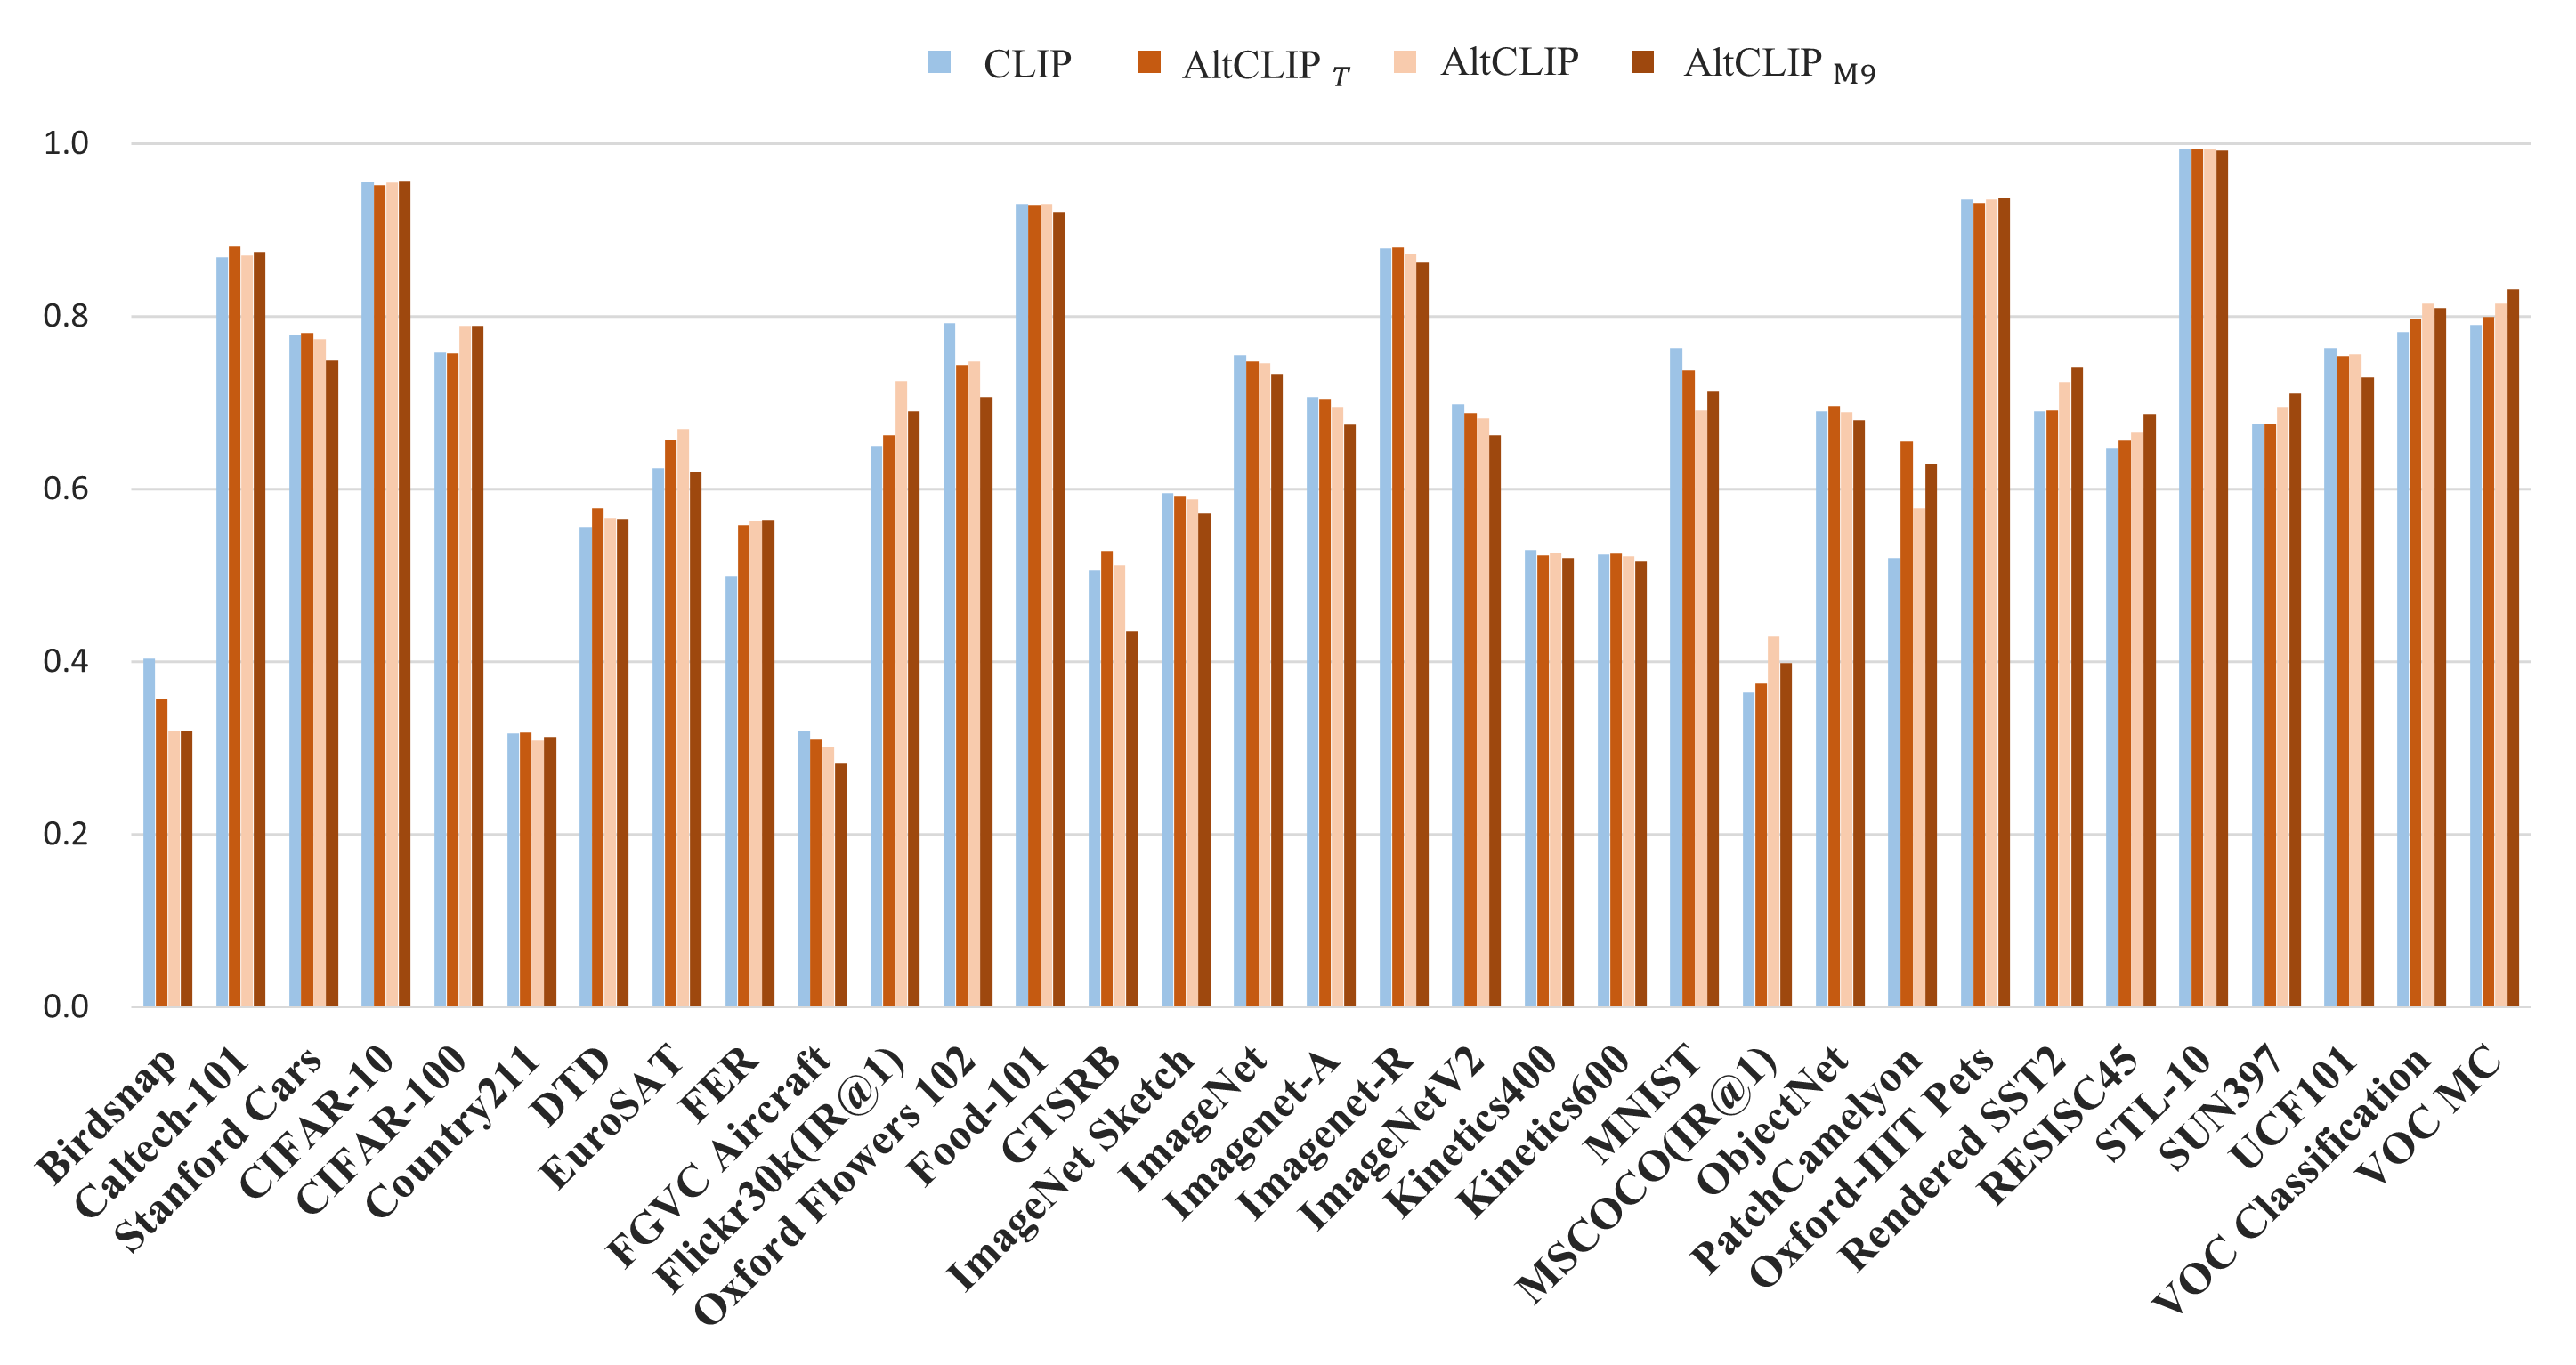
\includegraphics[scale=0.75]{figures/6_clipbcm}
    \caption{Comparison Results of our proposed model and OpenAI's CLIP. AltCLIP$_{T}$ denotes for our model after Teacher Learning Stage while AltCLIP denotes for our model after Contrastive Learning Stage. AltCLIP$_{M9}$ denotes for our model extending to 9 different languages. All image encoders are CLIP$_{ViT-L14}$. }
    \label{fig:clipbcm}
\end{figure*}
